\documentclass[titlepage, a4paper]{article}
\usepackage[english]{babel}
\usepackage[utf8]{inputenc}
\usepackage{graphicx}
\usepackage{color}
\usepackage{mathtools}
\usepackage{float}
\usepackage[parfill]{parskip}
\usepackage[margin=10pt,font=small,labelfont=bf,labelsep=endash]{caption}
\usepackage{epstopdf}
\usepackage{listings}
\epstopdfsetup{suffix=}
\DeclareGraphicsExtensions{.ps}
\DeclareGraphicsRule{.ps}{pdf}{.pdf}{`ps2pdf -dEPSCrop -dNOSAFER #1 \noexpand\OutputFile}

\lstset{literate=%
    {å}{{\r{a}}}1
    {ä}{{\"a}}1
    {ö}{{\"o}}1
    {Å}{{\r{A}}}1
    {Ä}{{\"A}}1
    {Ö}{{\"O}}1
}

\newcommand{\todo}[1] {\textbf{\textcolor{red}{#1}}}

\usepackage{fancyhdr}
\fancyhead[L]{}
\pagestyle{fancy}
\rhead{Alexander Yngve \\ Pål Kastman}
\chead{TDTS08}
\thispagestyle{empty}

\begin{document}

{\ }\vspace{45mm}

\begin{center}
  \Huge \textbf{TDTS08: Lab Report}
\end{center}
\begin{center}
  \Large Lab 1: Cache Memories
\end{center}

\vspace{250pt}

\begin{center}
  \begin{tabular}{|*{3}{p{40mm}|}}
    \hline
    \textbf{Name} & \textbf{PIN} & \textbf{Email} \\ \hline
           {Alexander Yngve} & {930320-6651} & {aleyn573@student.liu.se} \\ \hline
           {Pål Kastman} & {851212-7575} & {palka285@student.liu.se} \\ \hline
  \end{tabular}
\end{center}
\newpage

\tableofcontents
\thispagestyle{empty}
\newpage

\section{Introduction}
The purpose of this lab was to understand the functionality of cache memories, and to get an insight into various trade-offs related to the design of systems with cache memories.

We analyze caches in sizes ranging from 128kB to 4096kB and with associativity from 1 to 8.

\section{Cache basics}
\subsection{Problem 1}
\underline{How is a 8-bit memory adress divided into tag, line number and byte number?}

$$s = \text{log}_{2}(\text{no. of  blocks}) = \text{log}_{2}(64) = 6$$
$$r = \text{log}_{2}(\text{no. of lines in cache}) = \text{log}_{2}(8) = 3$$
$$w = \text{log}_{2}(\text{block size}) = \text{log}_{2}(4) = 2$$

$$\text{size of tag} = (s - r) = 3 \text{bits}$$
$$\text{size of line number} = r = 3 \text{bits}$$
$$\text{size of byte number} = w = 2 \text{bits}$$

\subsection{Problem 2}
\underline{Into what line would bytes with each of the following addresses be stored?}

000\underline{1 10}11 $\to$ line 6

001\underline{1 01}00 $\to$ line 5

110\underline{1 00}00 $\to$ line 4

101\underline{0 10}10 $\to$ line 2

\subsection{Problem 3}
\underline{Suppose the byte address 1010 0001 is stored in the cache.} \\
\underline{What are the addresses of the other bytes stored in the cache?}

1010 0000 \\
1010 0010 \\
1010 0011 \\

\subsection{Problem 4}
\underline{How many total bytes of memory can be stored in the cache?}

32 bytes

\subsection{Problem 5}
\underline{Why is the tag also stored in the cache?}

To associate the cacheline with an address and to calculate hit or miss.

\section{Locality of data}
Here we ran tests on two different architectures and with two different configurations.
cache1 has 1024 cachelines with each of them being 16 bytes long, its associativity being 1 which means it's directly mapped into the main memory.

cache2 also has 1024 cachelines with each of them being 8 bytes long, but its associativity is instead 2. This means that every memory cell in the main memory can store data into two different places in the cache, this means that cache1 and cache2 are still the same size.

Both caches are using the least recently used algorithm for deciding what data to store and what to overwrite.

The test files are doing the same thing but in different order, the test1 file is going through the array \textit{A} two times, the test2 file though is going through the list one time and first adding the value in position \textit{A[i]} and then the value in position \textit{A[i + CACHE\_SIZE]}. The test2 is going to cause a cache miss every time for cache1 since we are going outside the cache size every other time but for cache2 this won't be a problem since it has associativity 2 and therefore can save to two different places in the cache. For the test1 on the other hand, cache1 is going to perform better because we don't have to reload the cache as often, this can be seen in table \ref{tab:table1}.

This means that higher associativity is worse for higher spatial locality of data.



\begin{table}[H]
  \centering
  \caption{Miss rates}
  \begin{tabular}{|*{3}{p{20mm}|}}
    \hline
    \textbf{Miss rates} & {test1} & {test2} \\ \hline
           {cache1} & {0.0091} & {0.1577} \\ \hline
           {cache2} & {0.0177} & {0.0235} \\ \hline
  \end{tabular}
  \label{tab:table1}
\end{table}

\section{Evaluation of cache configurations}
Here we analyze how the cache memory performs when it only handles data, instructions and for both data and instructions.

\subsection{Description}
For the three test cases we tested with caches of size ranging from 128kB up to 4096kB. For each size in memory we also tested with associativity ranging from 1 to 8.

\subsection{Result}
We found that when only storing data in the cache, the smallest memory with the lowest associativity performed worst, and for every step in increasing the memory size and the associativity the performance also increased, this can be seen in figure \ref{fig:data-cache}.

\begin{figure}[H]
	\centering
	\scalebox{0.342}{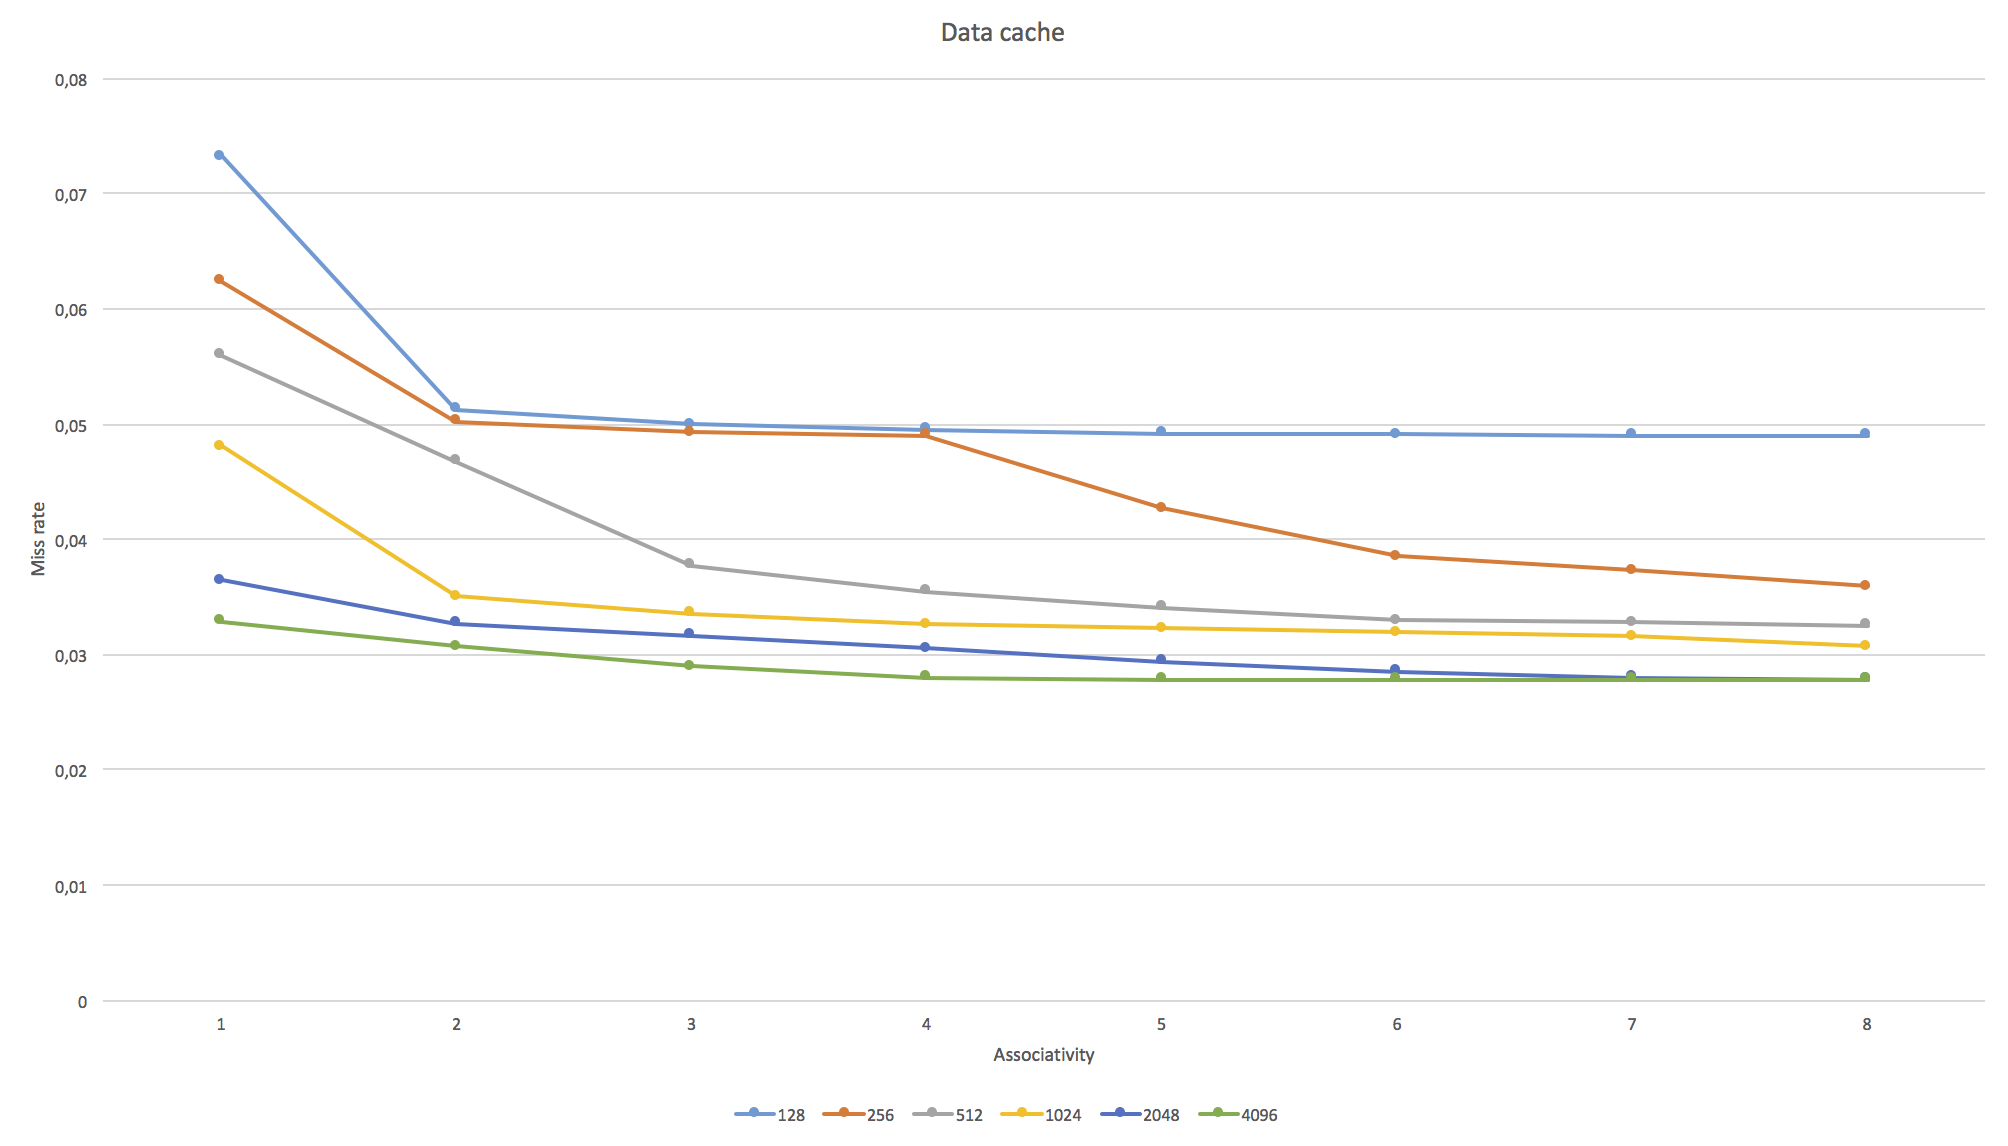
\includegraphics{img/data-cache.png}}
	\caption{Only data stored in cache.}
	\label{fig:data-cache}
\end{figure}

When storing only instructions in the cache, the same behaviour as when storing only data can be observed, this can be seen in figure \ref{fig:instruction-cache}.

\begin{figure}[H]
	\centering
	\scalebox{0.342}{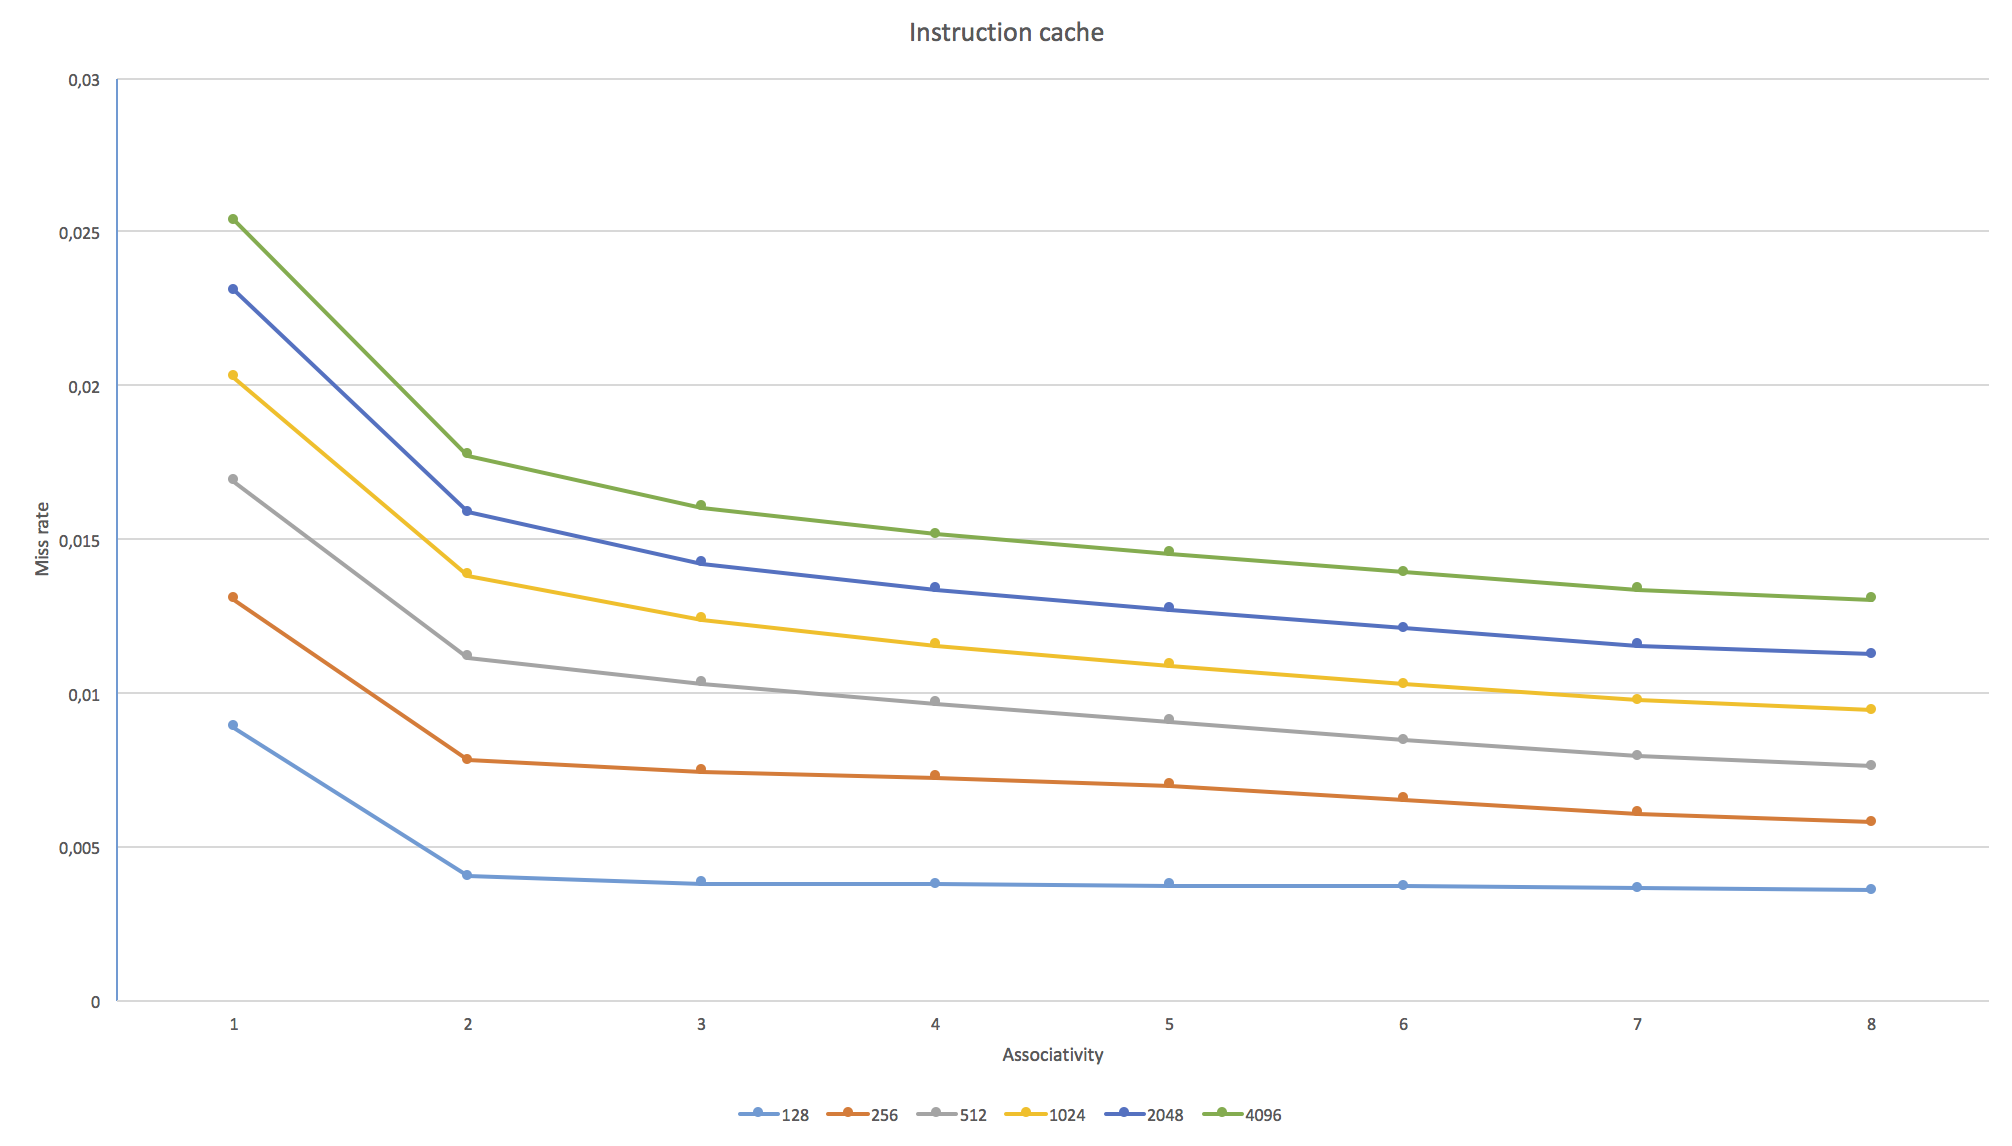
\includegraphics{img/instruction-cache.png}}
	\caption{Only instructions stored in cache.}
	\label{fig:instruction-cache}
\end{figure}

And finally when storing both data and instructions the biggest memory was again at the top in performance, with the gaps in performance decreasing with increasing size and associativity as can be seen in figure \ref{fig:unified-cache}.

\begin{figure}[H]
	\centering
	\scalebox{0.342}{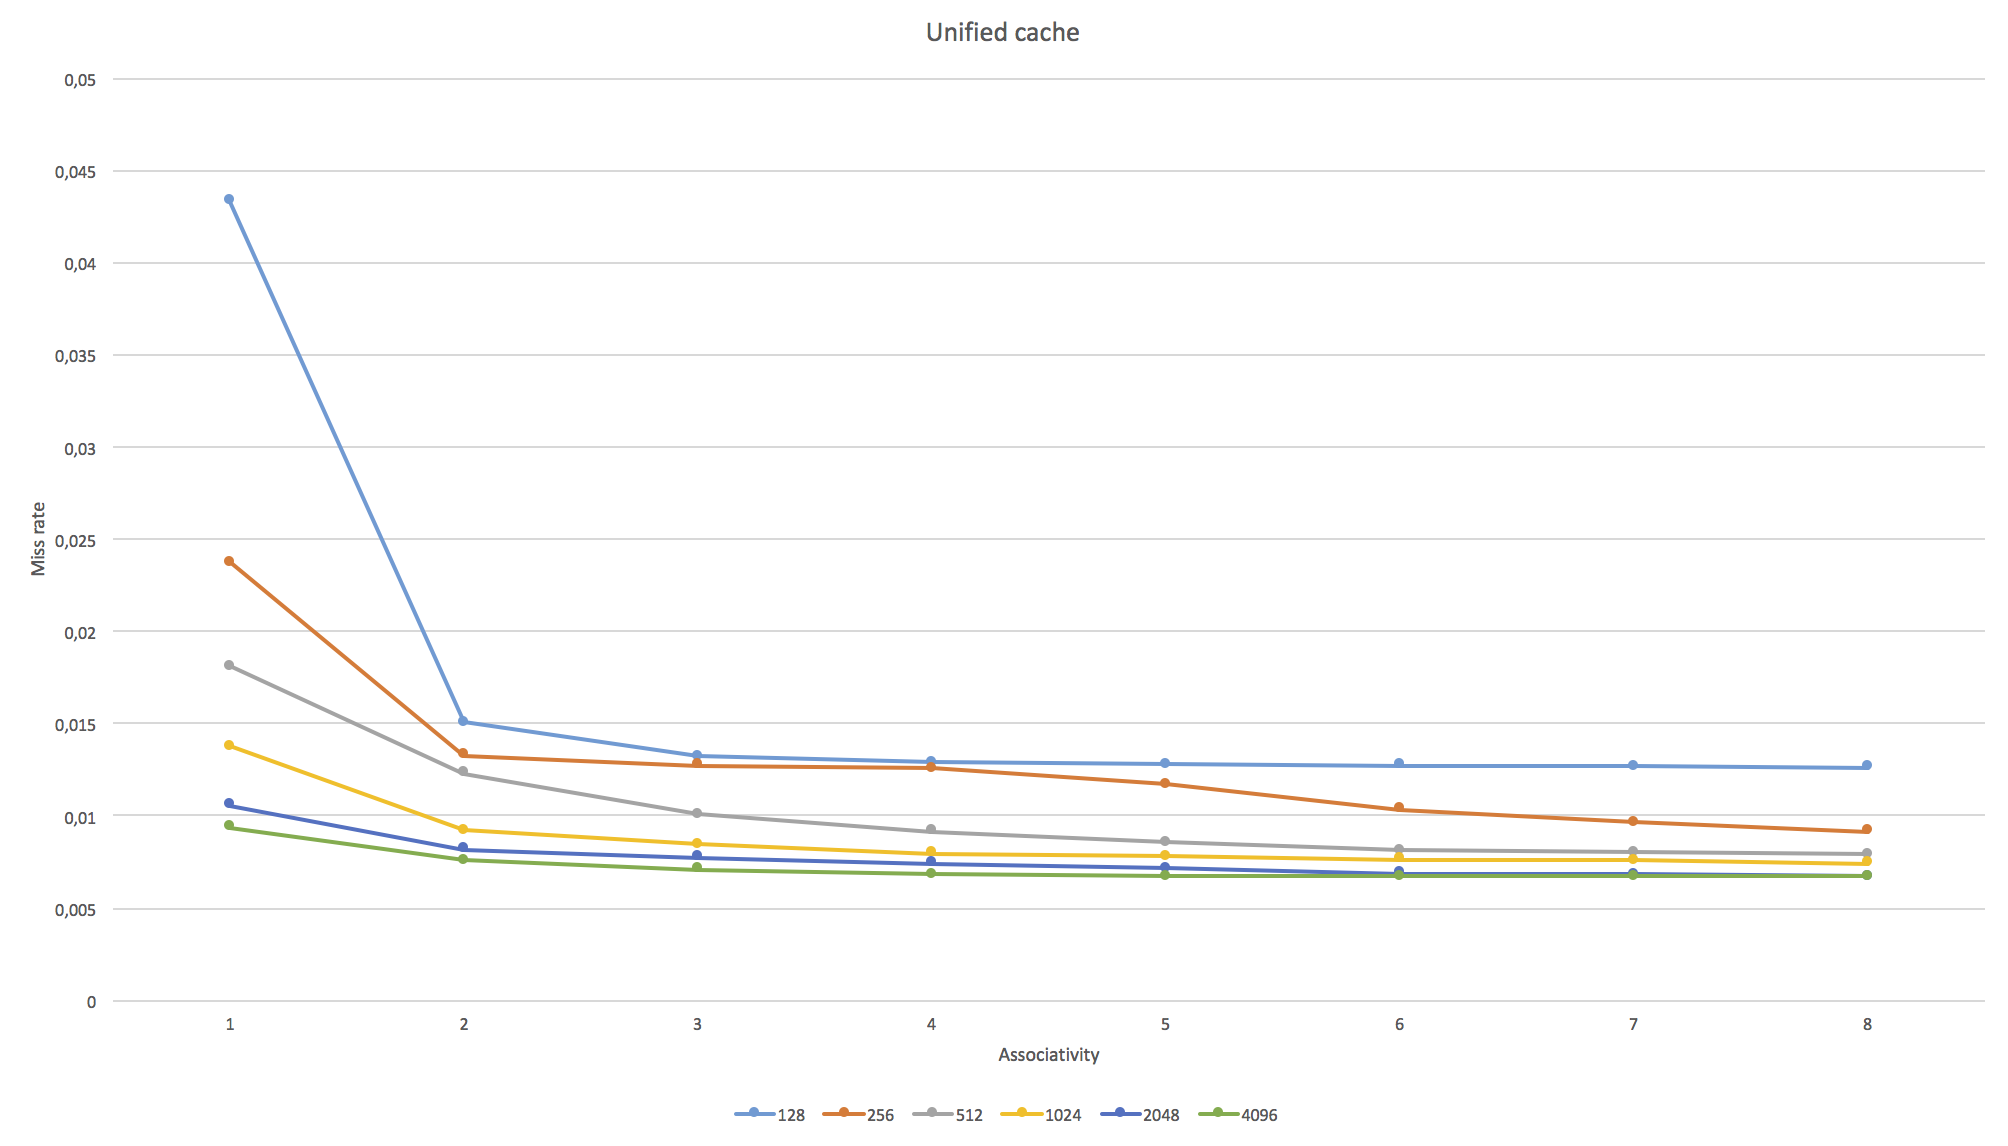
\includegraphics{img/unified-cache.png}}
	\caption{Both data and instructions is stored in cache.}
	\label{fig:unified-cache}
\end{figure}

We also noticed that the gap in performance tightened when the sizes and associativity of the caches became greater.

\section{Conclusion}
The miss rate for data is ten times higher than that for instructions which points to that the cache is big enough to store most of the instructions needed by the program, data access is the limiting factor.

We also notice that for instruction- and unified cache, associativity greater than two doesn't contribute that much. The size of the cache is therefore more important, as this gives a greater increase in performance.

To get the most optimal balance between associativity and size of the cache such evaluations is important, because if performance is not achieved by increasing associativity or size of the cache then you will have unnecessary costs. It's also important to do different benchmarks to get a balanced performance for different kind of programs, otherwise you could build a processor that only performs well in specific cases.

The conclusion is that as long as you have associativity equal or greater than two, you get more performance for your money by increasing the size of the cache than increasing associativity.

For example in this laboration we can see that for the unified cache we nearly don't achieve increase in performance if we increase the associativity, whereas for size of the cache the performance improves more.
\end{document}

